% Created 2014-03-19 Wed 03:24
\documentclass[11pt]{report}
\usepackage[utf8]{inputenc}
\usepackage[T1]{fontenc}
\usepackage{fixltx2e}
\usepackage{graphicx}
\usepackage{longtable}
\usepackage{float}
\usepackage{wrapfig}
\usepackage{rotating}
\usepackage[normalem]{ulem}
\usepackage{amsmath}
\usepackage{textcomp}
\usepackage{marvosym}
\usepackage{wasysym}
\usepackage{amssymb}
\usepackage{hyperref}
\tolerance=1000
\usepackage{minted}
\usepackage[bibstyle=numeric,citestyle=authoryear,backend=biber]{biblatex}
\addbibresource{bibliography.bib}
\usepackage[]{hyperref}
\usepackage[]{keystroke}
\hypersetup{hidelinks}
\usepackage[]{nomencl}
\usepackage{dirtree}
\usepackage[autostyle]{csquotes}
\author{Volker Strobel}
\date{\today}
\title{Knowledge Engineering Tools for Planning in PDDL - Syntax Highlighting, Task Generation and Plan Visualization and Execution - an extensible framework}
\hypersetup{
  pdfkeywords={},
  pdfsubject={},
  pdfcreator={Emacs 24.3.1 (Org mode 8.2.5h)}}
\begin{document}

\maketitle
\tableofcontents

\begin{abstract}
Automated planning and scheduling is a key component of artificial
intelligent (AI) behavior. A planning language that is widely used for
AI task specifications is the Planning Domain Definition Language
(PDDL). The aim of this project was to develop tools that simplify the
extensive knowledge engineering effort required by PDDL and thus
facilitate the construction of planning domains. For this purpose, an
extensible interface between the programming language Clojure and PDDL
was developed, that supports knowledge engineers in developing PDDL
projects. A tool based on this interface visualizes the type hierarchy
in PDDL domains, allowing knowledge engineers to keep track of the
domain structure and others that may have to work with the domains to
understand them at a glance. As further implementation of this
interface, a tool that calculates the distances of objects within a
problem file to each other was created to show the extent of this tool
and to present a way of bypassing PDDL's limited modeling capacity.
Lastly, a plug-in for the code editor Sublime Text was implemented to
aid developers with efficiently creating new PDDL file, navigating
within the code and with finding and fixing mistakes. In order to test
the quality of the syntax highlighter and the type diagram generator,
a user study was conducted with inexperienced PDDL users that were
asked to develop domains with and without the tools and to
subsequently evaluate the tools in regard to their usefulness and
usability. Both the time on task, number of errors and a post
questionnaire were analyzed and it was found that… All tools developed
within the scope of this thesis are unique in some regard and they can
all be altered very easily to work with other editors and planning
languages. An auxiliary tool to transform PDDL code into Clojure code
that was needed for the latter two tools, could be relevant for future
works in the field, as there are many additional use cases such as…

\url{https://www.ece.cmu.edu/~koopman/essays/abstract.html}
\end{abstract}
\chapter{Introduction}
\label{sec-1}
Assume you are a monkey in a cage. There are some bananas dangling
from the ceiling and a bunch of boxes lying around on the ground. You
are hungry and those bananas look delicious, but you just cannot reach
them. To solve the problem at hand it is important that you figure out
that the boxes can be stacked on top of each other and that you can
then climb on top of the boxes and reach the bananas, i.e. you need to
come up with a sequence of actions that take you from your initial
state to your goal state. This famous experiment is described by
Wolfgang Köhler in his book \citetitle{kohler1924mentality} and became
known (in a similar form) in Artificial Intelligence (AI) research as
the \emph{monkey and banana problem}. Importantly, with this experiment,
Köhler demonstrated that the monkeys did not acquire the solution by
trial and error, but rather that they actually understood the
environment enough to devise a plan only by contemplating the problem
in the context of their world. As can be seen from the scenario given
above, planning is a crucial component of problem-solving. However,
while monkeys and humans are able to create and continuously update
their mental models of the world thanks to sensors, AI implementations
are yet to fully master this skill (SOURCE! WHAT IS STILL MISSING?).
Thus, the most common and extensive approach to planning in AI to this
day is by means of knowledge engineering (KE). In KE, a human expert
that is familiar with the underlying syntax integrates world
information into a computer system \textcite{feigenbaum1983fifth}. In
automated planning, this is usually done using a planning language
applied in an editor. A standard Both the world and the problem are
modeled with the planning language and are then fed to the planning
software as inputs. The software produces the solution to the problem
in the form of a plan, that means a sequence of action, leading from
the initial state to the goal state as output. Naturally, the process
of creating these modeled worlds, from here on after called domains,
and problems is error-prone and time consuming. While it cannot be
denied that the planning systems are improving steadily as computer
processing times decrease and algorithms are altered to work even
better, the human factor in the knowledge engineering approach cannot
be ignored (SOURCE). Performances of planners are largely dependent on
the input they receive and the manner in which it is written (SOURCE).
Therefore, focusing on the usability of planning languages and hence
facilitating the knowledge engineering process is worthwhile. Although
recent PDDL extensions increased the expressiveness of PDDL and thus
allowed for real-world applications (SOURCE!!!), they also demand a
higher level of knowledge and attention on the part of the knowledge
engineer. Particularly during the first International Competition on
Knowledge Engineering for Planning and Scheduling in 2005, advances
were made in shifting the modelling process from a text-based to a
graphical programming environment. Even though such tools seem more
user-friendly at first, they also demonstrated considerable drawbacks
such as limited functionality, expenditure of time and editing
difficulty (SOURCE). Obviously, the usefulness of such tools depends
on the demands of the knowledge engineer. Yet, the question arises,
whether it is not better to develop tools that facilitate text-based
programming to such a degree that it is as easy to use as graphical
interfaces while still allowing the user full functionality and the
necessary insight into the code to edit it (Classification of Concrete
Textual Syntax Mapping Approaches - Nice Paper). As can be seen from
the two problems described above, tools that ensure greater usability
of planning language editors and thus help in producing standardized,
high-quality domains and problems that not only planners but also
other knowledge engineers can easily work with are greatly needed. The
main focus of this thesis is on the development of such handy tools
that support (and partially automate) the planning process. At first,
already existing planning tool are reviewed in order to put this
thesis in context. The body of this thesis consists of three parts.
The first part introduces the basics of planning and the PDDL syntax.
This is followed by the second part, which presents a extensible
interface between the programming language Clojure
\textcite{hickey2008clojure} and PDDL. Based on this interface, a
plug-in for the text and code editor Sublime Text (ST) was implemented
that consists of a type diagram generator and a distance calculator.
Furthermore, the development, application and customization of a
sophisticated syntax highlighter for ST will be presented. The third
part is devoted to the evaluation of the type diagram generator and
the syntax highlighter in terms of their usefulness and usability. As
means to this end, a small user study was conducted with subjects that
had no prior PDDL experience. The results and their implications will
be discussed before an outlook for future research and developments in
the field concludes this thesis (perhaps mention results and outlook
here). This thesis refers to deterministic planning and typed domains.

TODO: Add inspecting of domains as main focus of my work

\section{Finding of the research topic}
\label{sec-1-1}
During the research for this thesis, it turned out, that the tools for
writing and expanding extensive PDDL descriptions in a reasonable time
are limited, while tools for checking plans (\textcite{howey2004val} +
second topic, \textcite{glinsky2011visplan}) and applying PDDL
descriptions (broad range of planner)s, are far more matured. While
the original research interest was concentrated on possibilities and
limitations of artificial intelligence planning using PDDL, a focus
shift was performed, recognizing, that the main PDDL limitation is
still the \emph{basic} modeling process, meaning that efficient modeling of
useful domains and problems \emph{by hand} is hardly possible by the
existing tools (that's too hard!). Anymore, PDDL's general
representation ability is already limited through the missing support
of mathematical operations besides basic arithmetics. On this account,
a possibility for \emph{extending} PDDL was searched and found in Clojure,
using the relatedness of both languages embellished by PDDL's
LISP-derived notation. In the course of the development of this
PDDL/Clojure interface between great potential was seen for
facilitating the PDDL design process and thereby push the acceptance
and usage of PDDL in real world models. The customizability and
extensibility of the ST editor as well as the broad variety of
build-in editing features, constituted a convenient basis for the
design of a development environment for PDDL. A large variety of
language-independent plug-ins exist and is constantly developed, like
package managers, git connection . This project focuses the 
A key concept for the development was the ease of application, so that
new users should be able to effectively use the majority of functions
intuitively within a short time.
\chapter{Related Work}
\label{sec-2}
Related work primarily compromises knowledge engineering tools,
consisting of at least the possibility to edit PDDL files in a textual
environment and providing supporting functionality or checking the
correctness of PDDL.

\section{PDDL Studio}
\label{sec-2-1}
PDDL Studio \parencite{plch2012inspect}, is an application for
creating and managing PDDL projects. A project is regarded as a
collection of PDDL files. Its IDE is inspired by Microsoft Visual
Studio and imperative programming paradigms. Its core function is the
PDDL project management, consisting of managing PDDL projects and
creating, adding , so that corresponding as well as inspecting,
analyzing and modifying the underlying domain and problem files.
Besides general editing features like line counting, bracket matching
and auto-save, it supports PDDL specific editing features including
syntax highlighting, code folding (collapse code blocks to see only a
single visible line) and context aware code completions, all based on
a PDDL to XML parser. This parser can also be used to convert PDDL to
XML files and vice versa for domain and problem file editing. Also
based on this parser is a included, sophisticated on the fly error
detection, recognizing both syntax errors (missing keywords,
parentheses, etc.) and semantic errors (wrong type of predicate
parameters, misspelled predicates, etc.). As semantic errors can be of
a \emph{interfile nature}, meaning that there is a mismatch between domain
and problem file, PDDL Studio can detect such errors. TODO: Explain
further. The code completion feature allows for the selection of
completion suggestions for a for standard PDDL constructs and dynamic
list completions, that were used in the current project (TODO:
technical terms!). An interface allows the integration of command line
planners in order to run and compare different planning software. that
means syntax and semantic checking, syntax highlighting, code
completion and project management. While colors for highlighted code
can be customized, the background color of the tool is always white.
In its most recent version (of 15.6.2012), PDDL Studio's parser
supports PDDL 1.2, the official language of the first and second IPC
in 1998 and 2000 respectively. Since then, PDDL has largely evolved,
the most recent and most powerful version is PDDL 3.1, supporting
amongst others durative actions. PDDL Studio does not support the
insertion of larger code skeletons (called \emph{snippets} in this thesis).
The customization features (without editing the C source code) are
limited to the choice of font style and color of highlighted PDDL
expressions. PDDL Studio is written as standalone program, meaning
that there are no PDDL independent no extensions .
\section{itSIMPLE}
\label{sec-2-2}
The itSIMPLE project is a graphical interface that allows for
designing planning models in an object-oriented approach, using Unified
Modeling Language (UML) diagrams. UML was invented in order to
standardize modeling in software engineering (SE). It consists of
several part notations, the here presented tool uses the 'class
diagram' notation, as PDDL types and classes in OOP have strong
resemblance (see Tiago 2006, p 535). itSIMPLE proposes UML.P (UML in a
Planning Approach), a UML variant that specifies a structure for Class
(domain specification), Object (problem specification) and StateChart
Diagrams (dynamic behavior of actions).

itSIMPLE's main focus is to support knowledge engineers in the initial
stages of the design phase by providing an opportunity for the
transition of the informality of real world requirements to domain
models as formal specifications. The assertive statement is to provide
a tool for a \enquote\{disciplined process of elicitation, organization
and analysis of requirements\}. Petri Nets can be generated from the
UML model and be used to validate the planning domain's static and
dynamic bevahior. Finally, a PDDL representation can be generated from
the UML diagram, if required, edited, and finally used as input to a
variety of planning systems. The generated plan can be inspected using
the in-build plan analysis, consisting of a plan visualization and
plan simulation (TODO: write some more info). itSIMPLE's mdoeling
workflow is unidirectional, as changes in the PDDL domain do not
affect the UML model and UML models have to be modeled manually,
meaning that they cannot by generated using PDDL.

Starting in version 4.0 (currently in beta status as of writing of
this thesis) itSIMPLE expanded its features to allow the creation of
PDDL projects from scratch (i.e. without UML to PDDL translation
process). Thus far, the PDDL editing features are basic (see YouTube
video). A minimal syntax highlighting feature recognizes PDDL keywords
and variables. Furthermore, itSIMPLE provides templates for PDDL
constructs (similar to the code snippets presented in this thesis),
consisting of requirement specifications, predicates, actions, goals
and initial definitions. 

itSIMPLE's original and main design approach is reversed to the
process presented in this paper. While itSIMPLE generates PDDL models
from UML specifications, myPDDL generates type diagrams from PDDL. So,
while itSIMPLE focuses on the initial design phase, the tools
presented here are made for later stages.

However, \textcite{tonidandel2006reading} describe a translation
process, similar to the approach in this thesis, from a PDDL domain
specification to an object-oriented UML.P (UML in a Planning Approach)
model as possible integration for itSIMPLE. According to an email from
This translation process has not been fully implemented to date /
there is no release with this feature. 

This translation process does consider the order of variables as an
indicator for the importance.

\emph{Create\(_{\text{specializations}}\)} is the function for creating the typing
diagram. \emph{Create\(_{\text{associations}}\)} creates binary associations between
classes, whereby the first argument is considered as the \emph{main
argument}. 
This process requires semantic assumptions: the first argument of 

In an e-mail to, Tiago Vaquero (one of the authors), on February 28,
2014,, affirms that, the translation is not functional yet.

Currently there exists no implementation from PDDL to UML. UML.P's
semantic associations, 


myPDDL allows for a representation of a arbitrary, n-ary predicates,
without .
On the one hand, one the other hand, this enables the visualization of
n-ary predicates.

itSIMPLE's modeling process is focused on a graphical design
process and the newly added PDDL editing features are basic,
consisting of highlighted keywords and variables. The templates
primarily insert PDDL keywords, without showing the required syntax.
It is not possible to define custom key shortcuts. itSIMPLE is not
customizable (without editing the Java source code). There is no
possibility to show line numbers, matching brackets or code folding.

myPDDL shell support initial creating of domains (by code snippets)
and checking for validity of domains and problem by the type
generator.
\section{PDDL-Mode for Emacs}
\label{sec-2-3}
PDDL-mode (announced 2005 in a mailing list) is a major Emacs mode for
browsing and editing PDDL 2.2 files. It provides syntax highlighting
by basic pattern matching of keywords (and variables ?), regardless of
the current context. automatic indentation and completions and bracket
matching. Code snippets for the insertion of domains, problems and
actions are provided. A declaration menu shows all actions and
problems in the current PDDL file.

Being an Emacs mode, PDDL-mode is highly and easily customizable. Text
editor features, like auto-completion, can be extended independently
of this mode, by installing further Emacs modes.

\emph{myPDDL} uses Sublime Text, an editor, that is extensible and
customizable as well. The syntax highlighting feature of \emph{myPDDL}
supports all PDDL versions, up to the most recent version 3.1. in
contrast to \emph{PDDL-mode}, \emph{myPDDL-h's} syntax highlighting feature is
context-dependent and more extensive, as it can recognize almost any
PDDL construct and highlight it according to its semantic.

By syntax highlighting, both tools can support code navigation,
however, \emph{PDDL-mode} does not allow for an fast and evident error
detection.
\section{Conclusion \& Summary}
\label{sec-2-4}
As it can be seen, there is need for an up-to-date, customizable, text
editor with PDDL support, that supports the current standard PDDL 3.1. 
\chapter{Planning Basics and PDDL}
\label{sec-3}

Introduction to planing:
\url{http://books.google.de/books?id=eCj3cKC_3ikC&printsec=frontcover&dq=automated+planning&hl=en&sa=X&ei=3wgNU5fQIcHx4gSTsoDABA&redir_esc=y#v=onepage&q=automated%20planning&f=false}

Classical Planning!


Action planning plays a key role in artificial intelligence. Ranging
from the control of a (intelligent) household robot (or video game
enemy) to the operational procedure of a complex \ldots{} , instances of
planning tasks can possibly improve and automate work sequences. AP
provides reasons for the choice of actions and the coherent
deliberation process. By means of a formalization of a planning world
by the state space (predicates \& actions - operations), AP's
declared aim is to generate a sequence of these actions (a \emph{plan})
that can change the predicate values, from an initial state to a goal
state, both specified by the value of predicates.

\begin{itemize}
\item PDDL: Levels of expressivity (level 1 .. 4)
\item Formal description of PDDL tasks
\end{itemize}

Following this definition, in PDDL this there would be three parts:planner and use the generated solution file (\emph{plan}).

The planning domain definition language (PDDL) is a formal language
and the quasi standard for the description of planning tasks.  
PDDL was first described in PDDL-the planning domain definition
language (1998) and has been in constant development since then, .
This thesis makes use of \textcite{pddl3.1} if not otherwise stated. 

PDDL planning task specifications are composed of two separate files:

\begin{itemize}
\item Domain file: description of general types, predicates, functions
and actions -> uninstanciated problem independent
\item Problem file: description of a concrete problem environment -> instance specific
\end{itemize}


This separation allows for an intuitive process of task modeling:
While general instances are described in the domain file, specific
instances of problems are created in the problem files.

TODO: Add predicates and actions to domain, 
init and goal to problem and sequence of actions to plan
\begin{figure}[htb]
\centering
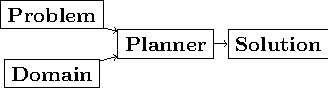
\includegraphics[width=.9\linewidth]{../img/pddl-workflow.pdf}
\caption{\label{fig:workflow}PDDL Planning workflow}
\end{figure}
The PDDL worklow. domain.pddl and problem.pddl represent typical
planning specification files, with the standard file extension \emph{.pddl}


This thesis is concerned with deterministic planning.

The syntax of basic constructs of these two files shell be investigated
further in this section. More complete descriptions as well as a
formulations in Backus-Naur form (BNF) can be found in
\textcite{fox2003pddl2} for PDDL 2.2 and \textcite{kovacs2011bnf} for
PDDL 3.1. 

\section{Domain File More scientific?}
\label{sec-3-1}

\begin{verbatim}
(define (domain name)
    
  (:requirements :requirement1
                 :requirement2...)

  (:types subsubtype1 subsubtype2 – subtype1
          subtype1 – type1
          subtype2 – type2
          ...
          type1 type2 …  - object)
  
  (:predicates (predicateName1 ?var1 – typeOfVar1)
               (predicateName2 ?var2 – typeOfVar2 ?var3 – typeOfVar3)
               ...)
     
  (:action actionName1
    :parameters (...)
    :precondition (...)
    :effect (...))
  
  (:action actionName2
    :parameters (...)
    :precondition (...)
    :effect (...))
    
...)
\end{verbatim}

The domain file contains the frame for planning tasks and determines,
which types and predicates are available and which actions are possible.

(Usually, domain files have a strict format: All keyword arguments must appear
in the order specified in the manual (an argument may be omitted,
according to 1998, only the strict part requires this order) and
just one PDDL definition (of a domain, problem, etc.) may appear per
file (same here). \cite[6]{fox2003pddl2}.)

The in Example 1 declared domain shell be explained by an example.

\subsection{Define}
\label{sec-3-1-1}
Every domain file starts with (define (domain NAME) \ldots{}) where,
NAME is a string that starts with a character, and then contains
further characters, number, hyphens (-) or underscores (\_).  
\subsection{Requirements}
\label{sec-3-1-2}
The requirements part is not a mandatory part of a PDDL domain file.
However, PDDL supports different "levels of expressivity", that means
subsets of PDDL features \textcite[1]{mcdermott1998pddl}. As most
planners only support a subset of PDDL the requirements part is useful
for determining if a planner is able to act on a given problem. They
are declared by the \verb~(:requirements ...)~ part. Some often used
requirements include \verb~:strips~ and \texttt{:typing}. Lists of requirement
flags and their meaning can be found in \textcite{fox2003pddl2} for
PDDL 2.1 and \textcite{kovacs2011bnf} for PDDL 3.1 It should be
mentioned, that almost no planner supports every part of PDDL.
\subsection{Types}
\label{sec-3-1-3}

In the \texttt{(:typing ...)} part, PDDL allows for structuring and typing
the domain. Typed lists are used to assign types to entity lists.
Relations can be expressed by a type hierarchy. whereby types can be
subtypes of Like that, parameters in actions can be typed, as well as
arguments in predicates, functions [extra source!]. Later, in the
problem file, objects will be assigned to types, like objects to
classes in Object Orientated Programming (OOP). Adding to the
(:requirement \ldots{}) part of the file guarantees, that typing can be
correctly used. Strips (no types) vs ADL (types).

Copied:
A typed list is used to declare the types of a list of entities; the
types are preceded by a minus sign (\-"), and every other element of
the list is declared to be of the rst type that follows it, or
object if there are no types that follow 

If order to be able to use type hierarchys in a domain file, the
requirement :typing should be declared (TODO: is :adl enough?).

\begin{verbatim}
(:types subsubtype1 subsubtype2 – subtype1
        subtype1 – type1
        subtype2 – type2
        ...
        type1 type2 …  - object)
\end{verbatim}

Every PDDL domain includes the built-in types \texttt{object} and \texttt{number},
whereby every defined type is subtype of \texttt{object}. 
\subsection{Actions}
\label{sec-3-1-4}

Actions are the tools for 

PDDL 3.1 supports two types of actions: durative-action and the
'regular' action.
\subsection{Functions}
\label{sec-3-1-5}
Functions are not supported by many planners (source!) and, before
PDDL 3.1 they could only be modeled as 

It is notable that before PDDL 3.0 the keyword functors was used instead
\section{Problem File}
\label{sec-3-2}

Problems are designed with respect to a domain. Domains usually have
multiple problems p01.pddl, p02.pddl, \ldots{} Problems declare the initial
world state and the goal state to be reached. They instantiate types,
in they way that they create objects 
\section{Planning}
\label{sec-3-3}

A planning solution is a sequence of actions that lead from the
initial state to the goal state. PDDL itself does not declare any
uniform plan layout.

The input to the planning software is a domain and a belonging
problem, the output is usually a totally or partially ordered plan.
Due to the yearly ICAPS, there is a broad range of available planners.
This thesis uses the planner SGPLAN\(_{\text{6}}\) \textcite{hsu2008sgplan}, a
'extensive' (in the sense of its supporting features) planner for both
temporal and non-temporal planning problems.

An overview of different planners is given at
\url{http://ipc.informatik.uni-freiburg.de/Planners}.



Additionally, the
quality of error messages is very diversified. While some simple
state: error occured, other list the problem and the line.

\chapter{Software Engineering Tools for AI Planning}
\label{sec-4}
\section{Statement of Problem}
\label{sec-4-1}

Writing and maintaining PDDL files can be time-consuming and
cumbersome \textcite{li2012translating}. So, the following development
tools shell support and facilitate the PDDL task design process and
reduce potential errors.

Below, methods are presented for

\begin{description}
\item[{Syntax Highlighting and Code Snippets}] Environment for Editing
PDDL files
\item[{Class Diagram Generator}] The automation of the PDDL task design process. File
input and output and dynamic generation (design level)
\item[{Human Planner Interaction}] An interactive PDDL environment: speech synthesis and
recognition.
\item[{Problem Generator}] Mathematical limitations (design level)
\end{description}

\section{Clojure Interface}
\label{sec-4-2}
\subsection{Approach}
\label{sec-4-2-1}
PDDL, as planning language modeling capabilities are limited, a
interface with a programming is handy a can reduce dramatically the
modeling time. In IPC, task generators are used write extensive domain
and problem files. As PDDL is used to create more and more complex domains
(SOURCE1, SOURCE2, SOURCE3, \ldots{}). 

While it seems to be reasonable to further extend PDDL's modeling
capability to at planning time instead of modeling time, a modeling
support tool as preprocessor is appropriate in any case
(\url{http://orff.uc3m.es/bitstream/handle/10016/14914/proceedings-WS-IPC2012.pdf?sequence=1#page=47})

As PDDL's syntax is inspired by LISP \parencite[64]{fox2003pddl2},
using a LISP dialect for the interface seems reasonable as file input
and output methods can use s-expressions instead of regular
expressions. This thesis uses Clojure \parencite{hickey2008clojure}, a
modern LISP dialect that runs on the Java Virtual Machine. So, PDDL
expressions can be extracted and written back in a similar manner, and
parts of PDDL files can be accessed in a natural way.

In this section, a general approach for generating PDDL
constructs, but also for reading in PDDL files, handling, using and
modifying the input, and generating PDDL files as output.
\subsection{Create}
\label{sec-4-2-2}
The functionality of sublime-PDDL is available trough a command line
interface, which allow for an integration of ST (and every other tool
that holds an interface for command line). Different tasks can be
performed by passing appropriate. New PDDL projects can be generated
by invoking the following command:
\begin{minted}[]{bash}
$ java -jar path/to/pddl.jar new NAME
\end{minted}
This will create a new structured project folder, consisting of a
domain and problem file with basic skeletons, a \texttt{domain} and \texttt{problem}
folder for an offline version control and a \texttt{png} and \texttt{dot} folder for
the generated dot language and png type diagrams respectively. This
approach should support an structured and organized design process,
and should finally lead to a standardized method for a PDDL project
structure in the planning community. This directory organization is
intended to contain just of couple of domain files in one project
keeping domain file per project, stored in the project root directory,
while problem files are stores in the subfolder problems. This
organization corresponds to the PDDL 

\dirtree{%
.1 NAME.
.2 dot.
.2 diagrams.
.2 domains.
.2 problems.
.2 solutions
.2 domain.pddl.
.2 p01.pddl.
.2 README.md.
}


\subsection{Basics}
\label{sec-4-2-3}
Through the higher-order filter method in Clojure, parts of PDDL files
can be easily extracted. Like that, one can extract parts of the file
and handle the constructs in a Clojure intern way.

As an example, the type handling will be represented here, but the
basic approach is similar for all PDDL constructs.

The here developed tools should be platform independent with a
development focus in UNIX/Linux systems, as most planners (source!)
run on Linux.
\subsection{Functions}
\label{sec-4-2-4}
As functions have a return value, the modeling possibilities
dramatically increase.

\subsection{Numerical Expressiveness}
\label{sec-4-2-5}
One might assume that the distance could be modeled as follows:

\begin{verbatim}
(durative action ...
...
  :duration (= ?duration (sqrt (coord-x )))
...
\end{verbatim}

However, PDDL does only support basic arithmetic operations (+, -, /, *).

An Euclidean distance function that uses the square root would be
convenient for distance modeling and measurement. However, PDDL 3.1
supports only four arithmetic operators (+, -, /, *). These
operators can be used in preconditions, effects
(normal/continuous/conditional) and durations.
\textcite{parkinson2012increasing} describe a workaround for this
drawback. By declaring an action `calculate-sqrt', they bypass the
lack of this function and rather write their own action that makes use
of the Babylonian root method.

\begin{enumerate}
\item Alternative \#1: Only sqrt exists
\label{sec-4-2-5-1}
Assuming that a function sqrt would actually exist, the duration could be modeled as follows:

\begin{verbatim}
:duration (= ?duration 
             (sqrt
              (+
               (*
                (- (pos-x (current-pos))
                   (pos-x ?goal))
                (- (pos-x (current-pos))
                   (pos-x ?goal)))
               (*
                (- (pos-y (current-pos))
                   (pos-y ?goal))
                (- (pos-y (current-pos))
                   (pos-y ?goal))))))
\end{verbatim}
\item Alternative \#2: sqrt and expt exist
\label{sec-4-2-5-2}
Assuming that a function sqrt would actually exist, the duration could be modeled as follows:
\begin{verbatim}
:duration (= ?duration 
             (sqrt
              (+
               (expt
                (- 
                 (pos-x (current-pos))
                 (pos-x ?goal)))
               (expt
                (- 
                 (pos-y (current-pos))
                 (pos-y ?goal))))))
\end{verbatim}

\item Alternative \#3: Calculate distance and hard code it, e.g. (distance table kitchen) = 5.9
\label{sec-4-2-5-3}

\begin{itemize}
\item Distance Matrix
\item \url{http://stackoverflow.com/questions/20654918/python-how-to-speed-up-calculation-of-distances-between-cities}
\item Scipy.spatial.distance (-> Clojure?)
\item Mention that the Taxicab geometry allows different ways that have an equal length
\end{itemize}

Another alternative is to make use of an external helper and, instead
of calculating every entry of the distance matrix. the distance only
if needed, incorporate every possible combination of two locations.
This approach has certainly a major drawback: With an increasing
amount of locations, the number of combinations increases
exponentially. That means, if there are 100 locations, there will be
\begin{center}
\fbox{
\begin{minipage}[c]{.6\textwidth}
TODO: Calculate possibilities

\rule[.8em]{\textwidth}{2pt}

nil\end{minipage}
}
\end{center}
\ldots{} . The native approach would be to iterate over the cities twice
and calculate only the half of the matrix (as it is symmetric, that
mean distance from A to B is the same as the distance from B to A).

\item Alternative \#4: Use the Manhattan distance
\label{sec-4-2-5-4}

Allowing the agent to move only vertically and horizontally would be
that one can use the so called Taxicab geometry (or Manhattan length)
as distance measurement.  In the Kitchen domain, this could be modeled
as follows:

\begin{verbatim}
% => Metric: reduce duration

% dKitchenware.pddl 
\begin{figure}[t]
\inputminted[mathescape, linenos, numbersep=5pt, frame=lines, framesep=2mm]
            {csharp}
            {Code/dKitchenware.pddl}
\caption{The basic kitchenware domain}
\end{figure}
\section
\end{verbatim}

\begin{center}
\fbox{
\begin{minipage}[c]{.6\textwidth}
TODO:

\rule[.8em]{\textwidth}{2pt}

TODO Human Planner Interaction
\end{minipage}
}
\end{center}
\end{enumerate}
\section{Syntax Highlighting and Code Snippets}
\label{sec-4-3}
\label{sec:syntax}


Writing extensive domain and problem files is a cumbersome task:
longer files can get quickly confusing. Therefore, it is convenient to
have a tool that supports editing these files. Syntax highlighting
describes the feature of text editors of displaying code in different
colors and fonts according to the category of terms (source: Wiki). A
syntax highlighting plug-in for the text and source code editors
\textcite{sublimetext2} and \textcite{sublimetext3} is proposed and
transferred to the on-line text editor Ace are used to implement this
feature, as ST Syntax Highlighting files can easily be converted to
Ace Files. 

Extending a available editor.
Furthermore, ST was used as it provides a framework for general code
editing. Features include code folding, 

For Mac user, TextMate (TM) is very similar to ST and the syntax
highlighting file can be used there, too. Besides, the general
principles (e.g. regular expressions) outlined here, apply to most of
other editors as well. So, a Pygments extension was written, that
allows for syntax highlighting in \LaTeX documents.


\subsection{Implementation and Customization}
\label{sec-4-3-1}
ST syntax definitions are written in property lists in the XML format.

For the ease of creation, the PDDL syntax highlighter is is
implemented by the use of the ST plug-in \textcite{aaapackagedev}. So,
the definitions can be written in YAML in converted to Plist XML later
on. \textcite{aaapackagedev} is a ST plugin, that helps
to create, amongst others, ST packages, syntax definitions and
'snippets' (re-usable code). 

By means of Oniguruma regular expressions \parencite{kosako}, scopes
are defined, that determine the meaning of the PDDL code block. ST
themes highlight different parts of the code through by the use of
scopes. Scopes are defined by the use of regular expressions (regexes)
in a tmLanguage file. The scope naming conventions mentioned in the
\citetitle{textmate} are applied here. By the means of the name, the
colors are assigned according to the current used ST theme. That means
that colors are not assigned per se, but dependently on the current
scheme. Through that, experienced users can use their default theme
and all can easily change the colors by changing the scheme. Different
ST themes display different colors (not all themes support all naming
conventions).

The syntax highlighting is intended for PDDL 3.1, but is backward
compatible to previous version. It's based on the Backus-Naur Form
(BNF) descriptions, formulated in
\textcite{kovacs2011bnf,fox2003pddl2,mcdermott1998pddl}.

The pattern matching heuristic that is implemented by the use of
regular expressions is used for assigning scopes to the parts of the
file. As a result of PDDL's LISP-derived syntax, PDDL uses the
s-expression format for representing information (SOURCE!). So, the
semantic of a larger PDDL part (sexpr) can be recognized by a opening
parenthesis, followed by PDDL keyword and finally matched closing
parentheses (potentially containing further sexpr). These scopes
allow for a fragmentation of the PDDL files, so that constructs are
only highlighted, if they appear in the right section.

The YAML-tmlanguage file is organized into repositories, so that
expressions can be re-used in different scopes. This organization also
allows for a customization of the syntax highlighter. The default 

The first part of the PDDL.YAML-tmlanguage
describes the parts of the PDDL task that should be highlighted. By
removing (or commenting) include statements, the syntax highlighter is
adjustable the user's need.

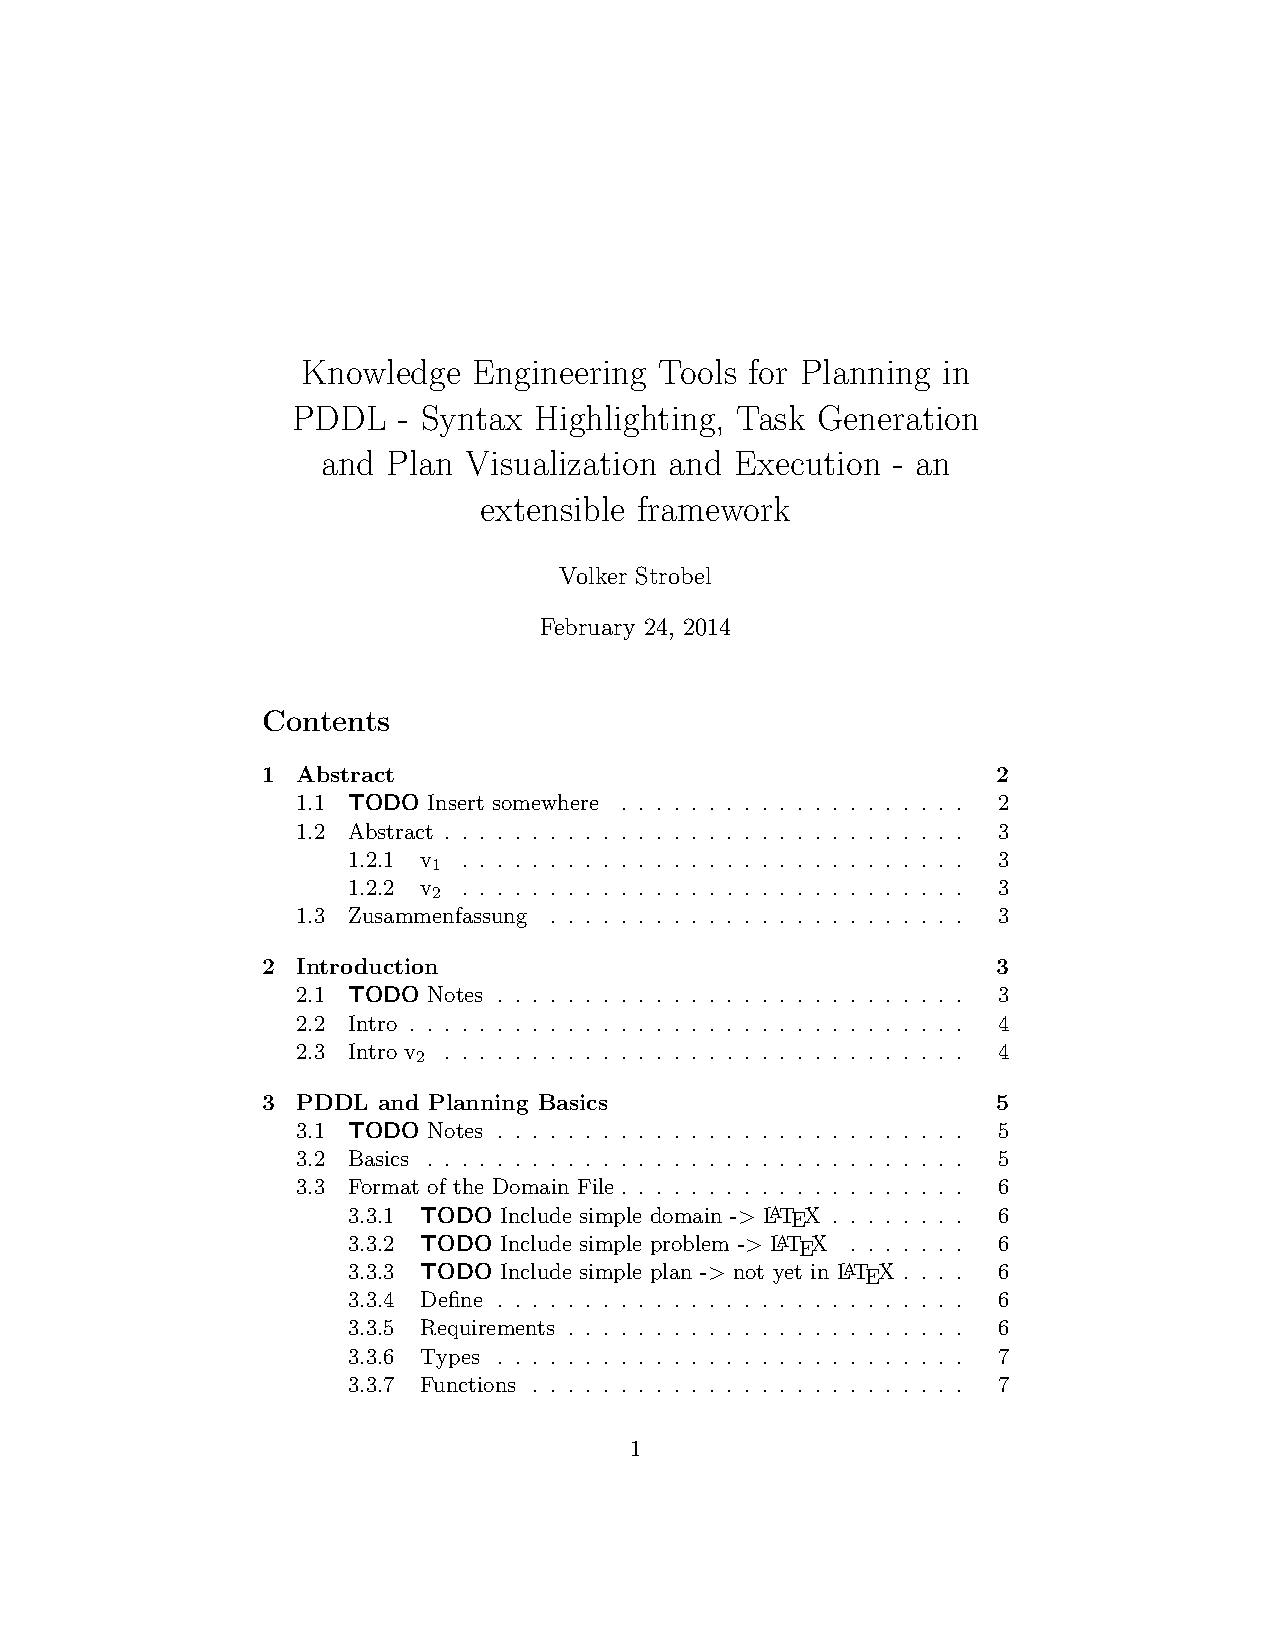
\includegraphics[width=.9\linewidth]{/home/pold/Pictures/ba.png}

\subsection{Usage and Customization}
\label{sec-4-3-2}

After invoking pddl.jar twice with 


To enable syntax highlighting and code snippets in ST, the files of
this repository have to be placed in the ST packages folder
(\url{http://www.sublimetext.com/docs/3/packages.html}). Following, the
features can be activated by changing ST's syntax to PDDL
(\texttt{View->Syntax->PDDL}).




By using ST as editor, language independent ST features are supported,
like auto completion of words already used in this file, code folding
and column selection, described in the Sublime Text 2 Documentation.



The PDDL.YAML-tmlanguage file is split in two parts:

By default, all scopes are included.
\subsection{Use case}
\label{sec-4-3-3}
Following, a small use case will be presented, that should represent a
typical work flow using the tools presented in this paper.

\begin{enumerate}
\item Initial Situation (Domain)
\label{sec-4-3-3-1}
Our world consists of two types of persons: hackers and non-hackers.
Hackers can be further divided into \emph{white hats} (seeking
vulnerabilities on behalf of the system owner), \emph{black hats}
(compromise security holes without permission) and \emph{gray hats}
(sometimes act legally, other times not). \emph{Software} can be
\emph{application} software, \emph{system} software or programming \emph{tools}.
System software can be further divided into drivers and operating
systems. A hacker must not be hungry (and in that case need some needs
some pizza) in order to exploit vulnerable software.
\item Problem
\label{sec-4-3-3-2}
\emph{Gary} is a \emph{hungry} \emph{white-hat} hacker who should exploit Gisela's vulnerable
\emph{application} software \emph{MysteriousTexMexMix} on behalf of her. In order to
plan the sequence of required actions, Gary uses the tools presented
in this paper and the planning software SGPlan\(_{\text{6}}\).
\item Workflow
\label{sec-4-3-3-3}
Gary creates a new PDDL project using the command line, to this end he
types
\begin{minted}[]{bash}
$ java -jar pddl.jar new hacker-world
\end{minted}
changes into that directory 
\begin{minted}[]{bash}
$ cd bulb-world
\end{minted}
and renames the file domain.pddl to 
\begin{minted}[]{bash}
$ mv domain.pddl garys-hacker-world.pddl
\end{minted}

To get an overview over the world structure, Gary doodles a quick type
diagram with the freely available graph editor and layout program yEd
(yFiles software, Tübingen, Germany) that represents the world and its
structure. Of course, he could also do this by pen and paper or using
any other graph editor.

[./gary\(_{\text{sketch.svg}}\) ]

He then opens this domain file in the Sublime Text 2 editor
\begin{minted}[]{bash}
$ sublime gary-hacker-world.pddl
\end{minted}
and starts to model his world. To this end, he uses the code snippets
\texttt{domain} for creating the domain skeleton, navigates inside the domain
file with \Tab, creates new type definitions with the snippets \texttt{t2}
and \texttt{t3}. After completing his first draft, he presses
\keystroke{f8}, for saving his file and displaying the PDDL type
diagram and sees the following diagram:

[.././hacker-world/diagrams/png-diagram3.png ]

He recognizes, that he forgot to model that system software can be
sub-divided into drivers and operating systems. Therefore he closes
the diagram and adds the missing type declaration. He continues to
write the PDDL domain and adds the required predicates with \texttt{p1} and
\texttt{p2}, for example he types

\keystroke{p}\keystroke{2}\Tab\keystroke{h}\keystroke{a}\keystroke{s}\Tab\keystroke{s}\Tab\keystroke{s}\Tab\keystroke{p}\Tab\keystroke{p}\Tab

And gets \texttt{(has ?s - software ?p - person)} and \texttt{action} for the action
definition.

The syntax highlighter shows Gary, if the uses incorrect PDDL syntax
or if the forgets to close a parenthesis, as then parts don't get
highlighted. 

A final check show that everything is as expected:

[.././hacker-world/diagrams/png-diagram3.png]

Gary knows, that the type diagram generator uses the Clojure
interface. So, adding \texttt{\#\_} just before the predicates s-expression
(that means \texttt{\#\_(:predicates ...)} excludes the predicates from the
type diagram, as this is the Clojure notation for commenting out
s-expressions (and more convenient than commenting every single line).
However, the \texttt{\#\_} construct is \emph{not} correct PDDL, so Gary generates
the diagram without the predicates, checks and sees that everything is
fine, removes the \texttt{\#\_}, saves and closes the file. 

The final version in the ST editor now looks like this:
[./domain2.pdf ]

In the command line, he now opens the PDDL problem file p01.pddl
\begin{minted}[]{bash}
$ sublime p01.pddl
\end{minted}
and adds the problem skeleton by typing \texttt{problem} and pressing \Tab.

The relevant output lines of the output file are

The planner SGPlan\(_{\text{5}}\) can be invoked by
\begin{minted}[]{bash}
$ ./sgplan -o garys-hacker-world.pddl \
           -f p01.pddl \
           -out plans/solution0.soln
\end{minted}
where -o specifies the domain file, -f the problem file and -out the
output file. 
The extension \texttt{.soln} for \texttt{solution0.soln} is used to show that solution
files are not specified by PDDL per se, however,
\cite[91]{fox2003pddl2} specifies plan syntax as a sequence of timed
actions. 

TODO: Possibly change planner to one that does not use time stamps.
\begin{verbatim}
0.001: (EAT-PIZZA BIG-PEPPERONI-PIZZA GARY) [1]
1.002: (EXPLOIT GARY MYSTERIOUS-TEX-MEX-MIX GISELA) [1]
\end{verbatim}

Gary now definitely knows, that he first has to eat the pepperoni
pizza, before he can exploit Gisela's application
\emph{MysteriousTexMexMix}.
The numbers to the left of the actions (\texttt{0.001}, \texttt{1.002}) and to the
right (both \texttt{[1]}) specify the start time and the duration of the
actions, respectively. They are dispensable in this case, as only the
sequence of actions is relevant.

The result directory tree looks as follows:
\dirtree{%
.1 NAME.
.2 dot.
.3 dot-diagram0.dot.
.3 dot-diagram1.dot.
.3 dot-diagram2.dot.
.2 diagrams.
.3 png-diagram0.png.
.3 png-diagram1.png.
.3 png-diagram2.png.
.2 domains.
.3 garys-hacker-world0.pddl.
.3 garys-hacker-world1.pddl.
.3 garys-hacker-world2.pddl.
.2 problems.
.2 plans
.3 plan0.soln
.2 domain.pddl.
.2 p01.pddl.
.2 README.md.
}

The generated files (\texttt{dot-diagram[0-2].dot}, \texttt{png-diagram[0-2].png},
\texttt{garys-hacker-world[0-2].pddl}) are the revision control versions,
generated each time the Clojure script is invoked (by pressing \keystrokes{F8}).

It can probably be seen, that this rather short description of the
world and in problem results in rather extensive PDDL files.
\end{enumerate}
\subsection{Evaluation}
\label{sec-4-3-4}
A key challenge of creating a sophisticated syntax highlighter without
the availability of a lexical parser, is the use of regular
expressions for creating a preferably complete PDDL identification.
While this a not possible by the expressiveness of regexes, this
syntax highlighter tries to come as close as possible.

The consistency and capability to highlight every PDDL construct in a
color according to its meaning, were checked by 320 (syntax
error-free) PDDL files, consisting of 87 domain and 230 problem files
(list of files). In that, no inconsistencies nor non-highlighted words
could be found.

While syntax highlighting can improve the time and ability to get
along in code files, it is mainly intended to distinct language
structures and syntax errors. 

\section{Type Diagram Generator}
\label{sec-4-4}
Graphical notations, have some advantages compared to textual
notations, as they simplify the communication between developers and
help to quickly grasp the connection of related system units (source!). 

But for all that one disadvantage has to be accepted: 

Object types play a major role in the PDDL design process: they are
involved, besides their definition in the \texttt{(:types ...)}, in the
constants, =(:predicates \ldots{}) and =(:actions \ldots{}) part. So, a fine
grasp of their hierarchy, as well as their involved predicates becomes
handy and assists knowledge engineers in the planning process.
Furthermore, in order to understand, use and extend available domains,
a crucial part is the grasping of types, their hierarchy, and the
predicates they that make use of them. Types strongly resemble classes
in object oriented programming,  as mentioned in chapter (\ldots{}), the type
definitions follow a specific syntax. For example \verb~truck car -
vehicle~ would indicate, that both \verb~truck~ and \verb~car~ are subtypes of
the super-type vehicle.

Subtypes and corresponding super-types can be extracted using regular
expressions (regex). The regex
\begin{verbatim}
#"((?:(?:\b[a-zA-Z](?:\w|-|_)+)\s+)+)-\s+(\b[a-zA-Z](?:\w|-|_)+)
\end{verbatim}
matches every kind of that form and a Clojure-friendly representation
in form of a hash-map can be created.

PDDL side ----------------------------------------------- Clojure side

'(:types \ldots{} \ldots{} --- \ldots{})                      \{\ldots{} [\ldots{} \ldots{} \ldots{}], \ldots{}\}

\begin{figure}[htb]
\centering
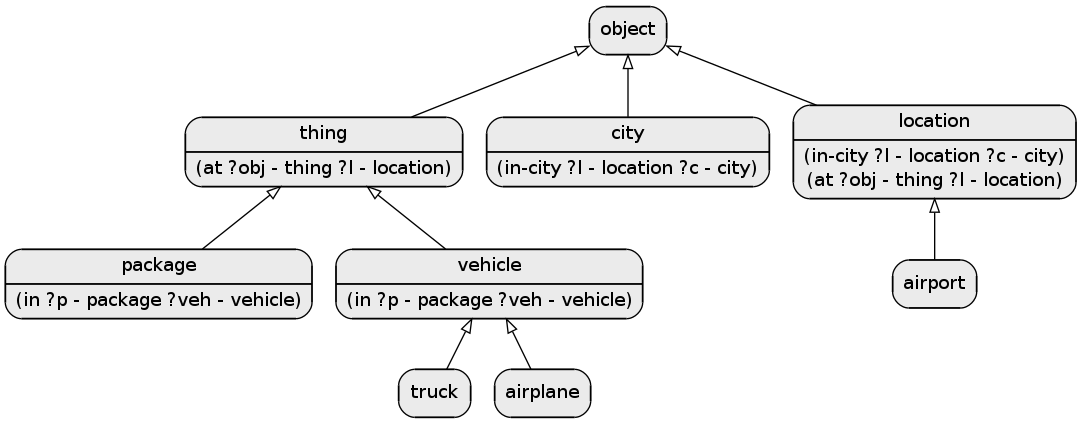
\includegraphics[width=.9\linewidth]{/home/pold/Documents/BA/org-ba/diagram.png}
\caption{Part of a PDDL domain and the corresponding, generated UML diagram}
\end{figure}
\chapter{Analysis}
\label{sec-5}
\section{Participants}
\label{sec-5-1}
Eight non-paid students (two female, Mean\(_{\text{age}}\)=23, SD\(_{\text{age}}\)=2) took part
in the experiment. All had knowledge about at least one LISP dialect,
and therefore about program code written as parenthesized lists, but
nobody one had faced PDDL prior to this study. One participant had
used the ST editor.  
\section{Material}
\label{sec-5-2}
The usability of myPDDL-s (Syntax Highlighter, see \ref{sec:syntax}) and
myPDDL-t (Type Diagram Generator, see \texttt{Type Diagram Generator}) were
tested. For this purpose, two domains (\emph{Planet Splisus}, \emph{Store}) with
fantasy type names were created. Participants were asked to answer
five questions that required to understand the PDDL type hierarchy.
Subjects were asked to work on questions, while time on task (per
question) was measured without subjects' knowledge, by asking the S to
say out loud the regarding answer. 

Furthermore, two deliberately incorrect domain files were provided to
the S, each containing 17 errors in total (consisting of X semantic
errors and Y syntax errors). Participants were asked to detect as many
errors as possible in six minutes and immediately correct found errors
in the code (as this could change the syntax highlighting of other
code parts) and write down the line and a description or the
correction of the error on a sheet of paper for an easy identification
in the analysis of test results.
\section{Design}
\label{sec-5-3}


\begin{center}
\begin{tabular}{l|llll}
\textbf{S} & \textbf{Order} &  &  & \\
\hline
A & \emph{Planet Splisus} & \emph{Logistics} & Store & Coffee\\
B & Store & Coffee & \emph{Planet Splisus} & \emph{Logistics}\\
C & Planet Splisus & Logistics & \emph{Store} & \emph{Coffee}\\
D & \emph{Store} & \emph{Coffee} & Planet Splisus & Logistics\\
E & \emph{Logistics} & \emph{Planet Splisus} & Coffee & Store\\
F & Coffee & Store & \emph{Logistics} & \emph{Planet Splisus}\\
G & Logistics & Planet Splisus & \emph{Coffee} & \emph{Store}\\
H & \emph{Coffee} & \emph{Store} & Logistics & Planet Splisus\\
\end{tabular}
\end{center}

\emph{Italic}: Tools part

\section{Procedure}
\label{sec-5-4}
At the earliest, 24 hours ahead testing date, participants received a
link to a 30-minute video tutorial and were asked to watch this video
before the test, if possible. This tutorial comprised a general
introduction to planning and a more specific introduction to PDDL's
domain syntax. In the video, participants were also asked to fulfill tasks
regarding PDDL and check theirs answers with the provided solutions in
the video. 

Upon arrival participants were asked to sign a consent form and to
take a set in front of a Laptop with a 13" display and a connected
monitor with a 17" display. If they did not already watch the PDDL
tutorial the participants first were asked to watch the tutorial then.
After that, any open questions regarding PDDL and the were clarified.

Immediately before the tools part, a three minute video introduction
to the functionality of myPDDL-syn and the usage of myPDDL-gen was
given. Subsequently, participants were asked to work on the tools
parts, meaning that participants were not confronted with the tools
before the actual test.
\section{Results}
\label{sec-5-5}
\begin{table}[htb]
\caption{Planet Splisus \textbf{Aggregated processing time of tasks with correct answers}}
\centering
\begin{tabular}{rll}
Task & Time & Points\\
\hline
1 &  & \\
2 &  & \\
3 &  & \\
4 &  & \\
5 &  & \\
\hline
Sum &  & \\
\end{tabular}
\end{table}



The questionnaire used The mean System Usability Scale (SUS) score was
XX, arguing for a high usability. 

\chapter{General Discussion}
\label{sec-6}

As seen in the conducted study, missing actions in the type diagram
can confuse. So, it is possibly helpful to exclude predicates in the
diagram and only display the plain type hierarchy (as all participants
were faster) before actions have not been added. Nevertheless, it is
worth noting that only PDDL novices were tested, after watching a
introduction video, without ever writing a domain by scratch.

Very likely, a learning effect will occur, so that tasks are more
easily to fulfill if they are done for the second time.
\chapter{Conclusion and Outlook}
\label{sec-7}
The tools (Clojure interface (I), type diagram generator (T), syntax
highlighting (S), distance calculation (C)) presented in this thesis
have been designed to support knowledge engineers in modeling planning
tasks as well as in understanding, modifying, extending and using
planning domains. The user study has been conducted to examine the
utility of I and T. There is some evidence that they can support
engineers in the design process, in particular in error detection and
in keeping track of the domain structure, the type hierarchy and
grasping predicates using these types. The faster understanding of the
domain structure could be beneficial for the maintenance and
application of existing domains and problems.  The communication
between engineers can be facilitated and

\section{Outlook}
\label{sec-7-1}
As

The plug-in for the editor ST could be further extended to provide
features of common integrated developing environments (IDE). A build
script for providing input to a planner for auto-matching domain and
matching problem(s) (or problem and matching domain) in ST could be
convenient.  
Detecting of semantic errors besides syntactic errors (as in PDDL
Studio) could be the next step to detecting errors fast and accurate.
Possible semantic errors could be undeclared variables or predicates
in a domain specification.
\section{Outlook}
\label{sec-7-2}
Besides ICKEPS, as mentioned in the introduction, also the yearly
workshop Knowledge Engineering for Planning and Scheduling (KEPS) will
promote the research in planning and scheduling technology.
Potentially, the main effort of for implementing models in planning
will be shifted from the manual KE to the automated knowledge
acquisition (KA). Perception systems, Nevertheless, a engineer who
double-checks the generated tasks will be irreplaceable.



\printbibliography

\chapter{Appendix}
\label{sec-8}

This code can also be found on the enclosed CD, and on the Internet
page \url{https://github.com/pold87/sublime-pddl} (most recent
version).

The website \url{http://pold87.github.io/sublime-pddl/} is the accompanying
website for this project.

\begin{minted}[]{clojure}
(ns org-ba.core
  (:gen-class :main true)
  (:require [clojure.tools.reader.edn :as edn]
            [clojure.java.io :as io]
            [clojure.pprint :as pprint]
            [dorothy.core :as doro]
            [rhizome.viz :as rhi]
            [clojure.math.numeric-tower :as math]
            [quil.core :as quil]
            [clojure.java.shell :as shell]
            [me.raynes.conch :as conch]
            [me.raynes.conch.low-level :as conch-sh]
            [fipp.printer :as p]
            [fipp.edn :refer (pprint) :rename {pprint fipp}]
            [me.raynes.fs :as fs])
  (:import [javax.swing JPanel JButton JFrame JLabel]
           [java.awt.image BufferedImage BufferedImageOp]
           [java.io File]))

(defn read-lispstyle-edn
  "Read one s-expression from a file"
  [filename]
  (with-open [rdr (java.io.PushbackReader. (clojure.java.io/reader filename))]
    (edn/read rdr)))

(defmacro write->file
  "Writes body to the given file name"
  [filename & body]
  `(do
     (with-open [w# (io/writer ~filename)]
     (binding [*out* w#]
       ~@body))
  (println "Written to file: " ~filename)))

(defn read-objs
  "Read PDDL objects from a file and add type
  (e.g. 'table bed' -> (list table - furniture
                        bed - furniture))"
  [file object-type]
  (as-> (slurp file) objs
        (clojure.string/split objs #"\s")
        (map #(str % " - " object-type) objs)))



(defn create-pddl
  "Creates a PDDL file from a list of objects and locations"
  [objs-file objs-type]
  (str
   "(define (domain domainName)

  (:requirements
     :durative-actions
     :equality
     :negative-preconditions
     :numeric-fluents
     :object-fluents
     :typing)

  (:types\n"
   (pprint/cl-format nil "~{~&~5@T~a~}" (read-objs objs-file objs-type))
   ")

  (:constants

  )

  (:predicates

  )

  (:functions

  )

  (:durative-action actionName
     :parameters (?x - <objectType>)
     :duration (= ?duration #duration)
     :condition (at start <effects>)
     :effect (at end <effects>))
)"
   ))

(defn split-up
  "Split a PDDL type list (:types obj1.1 obj1.2 - objT1 obj2 - objT2 ...)
  into strings of subtypes and associated types,
  [[subytype1 subtype 2 ... - type][subtype1 subtype2 ...][type]"
  [coll]
  ;; Remove ':types' if it is present.
  (let [coll (if (= :types (first coll))
               (rest coll)
               coll)]
    ;; Capturing group 1 is type1.1 type1.2.
    ;; Capturing group 1 is type1.
    (re-seq #"((?:(?:\b[a-zA-Z](?:\w|-|_)+)\s+)+)-\s+(\b[a-zA-Z](?:\w|-|_)+)"
            (clojure.string/join " " coll))))


(defn types->hash-map-helper
  "Convert splitted type list (['<expr>' '<subtype1.1> <subtype1.2> ...' '<type1>']
  to a hash-map {'<type1>': ['<subtype1.1>' '<subtype1.2>' ...], '<type2>': ...}"
  [coll]
  (reduce (fn [h-map [_ objs obj-type]]
            (let [key-obj-type (keyword obj-type)
                  existing-vals (key-obj-type h-map)]
              (assoc h-map
                key-obj-type
                (concat existing-vals
                        (clojure.string/split objs #"\s")))))
          {}
          coll))

(defn types->hash-map
  "Splits types and converts them into a hash-map"
  [pddl-types]
  (types->hash-map-helper (split-up pddl-types)))

(defn map-entry->TikZ-seq
  "Converts a hashmap entry (:key [val1 val2 ...])
to a TikZ string (key -- { val1, val2 })"
  [entry]
  (str
   (name (key entry))
   " -- "
   "{" (clojure.string/join ", " (val entry)) "}"))

(defn hash-map->TikZ-out
  "Converts complete PDDL type hash-map to TikZ file"
  [h-map]
  (str
   "\\documentclass[tikz]{standalone}

\\usepackage[utf8]{inputenc}

\\usepackage{tikz}

\\usetikzlibrary{graphdrawing}
\\usetikzlibrary{graphs}
\\usegdlibrary{layered,trees}

\\begin{document}

\\begin{tikzpicture}

\\graph[layered layout, nodes={draw,circle,fill=blue!20,font=\\bfseries}]
{
  " (clojure.string/join ",\n  " (map map-entry->TikZ-seq h-map))
  "
};

\\end{tikzpicture}
\\end{document}"))

(defn types-map-entry->dot-language
  "Converts one hash-map entry
to the dot language"
  [entry]
  (str
   "\"" (name (key entry)) "\""
   " -> "
   "{" (clojure.string/join " " (map #(str "\"" % "\"")  (val entry))) "}"))


(defn types-hash-map->dot-language
  "Converts a PDDL types hash-map
to the dot language notation"
  [pddl-types-map]
  (clojure.string/join "\n" (map types-map-entry->dot-language pddl-types-map)))

;;; Read PDDL predicates and generate UML 'type' diagram
(defn get-types-in-predicate
  "Takes a PDDL predicate,
  e.g. '(at ?x - location ?y - object)
  and returns the involved types, e.g.
  '(location object)"
  [pddl-pred]
  (remove
   (fn [s]
     (let [first-char (first (name s))]
       (or (= \- first-char)
           (= \? first-char)))) (rest pddl-pred)))

(defn pddl-pred->hash-map-long
  "Takes a PDDL predicate, e.g.
  '(at ?x - location ?y - object) and returns a
  hash-map, that assigns the involved types
  to this predicate, e.g.
  {location [(at ?x - location ?y - object)],
   object [(at ?x - location ?y - object)]}"
  [pddl-pred]
  (reduce (fn [h-map pddl-type]
            (assoc h-map
              pddl-type
              (list pddl-pred)))
          {}
          (get-types-in-predicate pddl-pred)))


(pddl-pred->hash-map-long '(at ?x - location ?y - object))

;;; TODO: Create short version wiht prolog predicate style
;;; e.g. at/2
(defn all-pddl-preds->hash-map-long
  "Takes a list of PDDL predicates and
  returns a hash-map of types and the
  assigned predicate"
  [pddl-preds]
  (let [pddl-preds (if (= :predicates (first pddl-preds))
                     (rest pddl-preds)
                     pddl-preds)]
    (apply merge-with concat
           (map pddl-pred->hash-map-long pddl-preds))))

(defn hash-map->dot
  "Converts a hash-map to
  dot language for creating
  UML diagrams"
  [h-map]  
  (map (fn [map-entry]
         (str (key map-entry)
              "[label = \"{"
              (key map-entry)
              "|"
              (clojure.string/join "\\l"  (val map-entry))
              "}\"]\n"))
       h-map))

(defn hash-map->dot-with-style
  "Adds dot template to
hash-map>dot"
  [h-map]
  (str
   "digraph hierarchy {
node[shape=record,style=filled,fillcolor=gray92]
edge[dir=back, arrowtail=empty]
\n"
   (clojure.string/join (hash-map->dot h-map))
   "}"))


(defn PDDL->dot-with-style
  "Adds dot template to
hash-map>dot"
  [preds types]
  (str
   "digraph hierarchy {
node[shape=record,style=filled,fillcolor=gray92]
edge[dir=back, arrowtail=empty]
\n"

   (clojure.string/join (hash-map->dot (all-pddl-preds->hash-map-long preds)))
   (types-hash-map->dot-language (types->hash-map types))

   "}"))

;;; Example for Predicate:
(def predicates 
  '(:predicates (at ?x - location ?y - object)
                (have ?x - object) 
                (hot ?x - object)
                (on ?f - furniture ?o - object)))

;;; Example invocation:
(hash-map->dot-with-style (all-pddl-preds->hash-map-long predicates))


(defn get-PDDL-construct
  "Takes a PDDL keyword and a PDDL domain/problem
file and returns all parts of the file that
belong to the PDDL keyword."
  [pddl-keyword pddl-file]
  (filter #(and (seq? %)
                (= (keyword pddl-keyword)
                   (first %)))
          (read-lispstyle-edn pddl-file)))


                                        ; TODO: Throw error if length != 1
(defn get-PDDL-predicates
  "Get all predicates in a PDDL file"
  [pddl-file]
  (first (get-PDDL-construct 'predicates pddl-file)))

(defn get-PDDL-init
  "Get all predicates in a PDDL file"
  [pddl-file]
  (first (get-PDDL-construct 'init pddl-file)))


                                        ; TODO: Throw error if length != 1
(defn get-PDDL-types
  "Get all types in a PDDL file"
  [pddl-file]
  (first (get-PDDL-construct 'types pddl-file)))

(defn PDDL->dot
  "Takes a complete PDDL file
and generates a UML type diagram"
  [pddl-file]
  (PDDL->dot-with-style (get-PDDL-predicates pddl-file)
                        (get-PDDL-types pddl-file)))

(defn PDDL->dot-commandline-input
  "Assumes that the PDDL input is
a string and 'reads' this string"
  [pddl-file]
  (print "The type is " (type pddl-file))
  (PDDL->dot (edn/read-string pddl-file)))


(defn PDDL->dot-file-input
  "Reads PDDL file"
  [pddl-file-name]
  (PDDL->dot pddl-file-name))

;;;; math helper functions

(defn sqr
  "Square of a number"
  [x]
  (* x x))

(defn round-places [number decimals]
  "Round to decimal places"
  (let [factor (math/expt 10 decimals)]
    (double (/ (math/round (* factor number)) factor))))

(defn euclidean-squared-distance
  "Computes the Euclidean squared distance between two sequences"
  [a b]
  (reduce + (map (comp sqr -) a b)))

(defn euclidean-distance
  "Computes the Euclidean distance between two sequences"
  [a b]
  (math/sqrt (euclidean-squared-distance a b)))

;;;; End math helper functions

(defn calc-distance-good
  "Calculates the distance and writes
the calculated distances to a string
IS VERY GOOD !!!"
  [locations]
  (for [[ _ loc1 & xyz-1] locations
        [ _ loc2 & xyz-2] locations]
    ;; Euclidean distance rounded to 4 decimal places.
    (list 'distance loc1 loc2 (round-places (euclidean-distance xyz-1 xyz-2) 4))))

(defn get-specified-predicates-in-pddl-file
  "Extracts all locations in the predicates part
(by the specified name) in a PDDL file"
  [pddl-file predicate-name]
  (filter #(and (seq? %)
                (= predicate-name (first %)))
          (get-PDDL-predicates pddl-file)))

(defn get-specified-inits-in-pddl-file
  "Extracts all locations in the init part
(by the specified name) in a PDDL problem"
  [pddl-file predicate-name]
  (filter #(and (seq? %)
                (= predicate-name (first %)))
          (get-PDDL-init pddl-file)))

(defn calc-distance
  "Calculate distances of PDDL objects"
  [locations]
  (for [[ _ loc1 & xyz-1] locations
        [ _ loc2 & xyz-2] locations]
    ;; Euclidean distance rounded to 4 decimal places.
    `(~'distance ~loc1 ~loc2
                 ~(euclidean-distance xyz-1 xyz-2))))

; LOOK UP: extended equality: 'hello = :hello

(defn add-part-to-PDDL
  "Takes a PDDL domain or problem
and add the specified part to the
specified position"
  [pddl-file position part]

  (map #(if (and (seq? %)
                 (= (keyword position) (first %)))
          (concat % part)
          %)
       (read-lispstyle-edn pddl-file)))

(defn find-new-file-name
  "Take a filename and determines, the new number
that has to be added to create a new file. E.g.
file1.img file2.img file3.img means that, file4.img
has to be created"
  [filename extension]
  (loop [n 0]
    (if-not (io/.exists (io/as-file
                         (str filename n extension)))
      (str filename n extension)
      (recur (inc n)))))


;;; Copied from https://www.refheap.com/9034
(defn exit-on-close [sketch]
  "Guarantees that Clojure script will be
exited after the JFrame is closed"
  (let [frame (-> sketch .getParent .getParent .getParent .getParent)]
    (.setDefaultCloseOperation frame javax.swing.JFrame/EXIT_ON_CLOSE)))


(defn extract-locations-from-file
  "Read a Blender LISP file and write object positions to out-file"
  [file-in file-out]
  (let [map-destructorer-local (fn [[_addgv _furniture object
                                      [_make-instance _object-detail
                                          _pose [_tfmps
                                                _type-name
                                                _type-num
                                                [_vector-3d x y z & more]
                                                & _more1]
                                       & _more2]]] (list "location" (name object) x y z))]
    (with-open [rdr (java.io.PushbackReader. (io/reader file-in))]
      (println
      (doall
          (map map-destructorer-local
               (filter #(and (seq? %) (= 'addgv (first %)))
                       (take-while #(not= % :end)
                                   (repeatedly  #(edn/read {:eof :end} rdr))))))))))


;; Main method
;; TODO: Command line options
(defn -main
  "Runs the input/output scripts"
  [& args]

  (cond
   ;; Create a new PDDL project
   (= "new" (first args))
   (let [project-name (second args)]
     (fs/mkdir project-name)
     (fs/mkdir (str project-name "/dot"))
     (fs/mkdir (str project-name "/diagrams"))
     (fs/mkdir (str project-name "/domains"))
     (fs/mkdir (str project-name "/problems"))
     (fs/create (io/file (str project-name "/domain.pddl")))
     (fs/create (io/file (str project-name "/p01.pddl"))))

   ;; -l flag for adding locations in PDDL file
   (= (second args) "-l")
   (let [content (add-part-to-PDDL (first args)
                                   'init
                                   (calc-distance-good
                                    (get-specified-inits-in-pddl-file (first args)
                                                                      'location)))
         new-filename (clojure.string/replace-first (first args)
                                                    #"(.+).pddl"
                                                    "$1-locations.pddl")] ; TODO: location as arg

     (write->file new-filename (pprint/pprint content)))


   ;; Write dot graph to file.
   :else
   (let [input-domain (first args)
         new-dot-filename (find-new-file-name "dot/dot-diagram" ".dot")
         new-png-filename (find-new-file-name "diagrams/png-diagram" ".png")
         input-domain-filename (fs/name input-domain)
         domain-version (find-new-file-name
                         (str "domains/" input-domain-filename) (fs/extension input-domain))]

     ;; Save input domain version in folder domains.
     (fs/copy+ input-domain domain-version)     

     ;; Create folders for dot files and png diagrams
     (fs/mkdir "dot")
     (fs/mkdir "diagrams")

     ;; Create dot language file in dot folder.
     (doall
      (write->file new-dot-filename
                   (print (PDDL->dot-file-input input-domain))))

     ;; Create a png file from dot
     (fs/exec "dot" "-Tpng" "-o" new-png-filename new-dot-filename)

     ;; Settings for displaying the generated diagram.
     (def img (ref nil))

     (defn setup []
       (quil/background 0)
       (dosync (ref-set img (quil/load-image new-png-filename))))

     (def img-size
       (with-open [r (java.io.FileInputStream. new-png-filename)]
         (let [image (javax.imageio.ImageIO/read r)
               img-width (.getWidth image)
               img-height (.getHeight image)]
           [img-width img-height])))

     (defn draw []
       (quil/image @img 0 0))

     ;; Display png file in JFrame.
     (exit-on-close
      (quil/sketch
       :title (str "PDDL Type Diagram - " input-domain-filename)
       :setup setup
       :draw draw
       :size (vec img-size))))))
\end{minted}
\begin{verbatim}
# [PackageDev] target_format: plist, ext: tmLanguage
---
name: PDDL
scopeName: text.pddl
fileTypes: [pddl]
uuid: 2aef09fc-d29e-4efd-bf1a-974598feb7a9

patterns:

#####################
### Customization ###

- include: '#domain'
- include: '#problem'
- include: '#comment'

##################
### Repository ###

repository:


##############################
### General specifications ###
##############################

  built-in-var:
    match: \?duration 
    name: variable.language.pddl

  variable:
    match: '(?:^|\s+)(\?[a-zA-Z](?:\w|-|_)*)'
    # name: variable.other.pddl
    name: keyword.other.pddl # TODO: changeback again to variable.other.pddl
    # this is just a dirty hack for highlighting

  pddl-expr:
    match: '(?:^|\s+)([a-zA-Z](?:\w|-|_)*)(?!:|\?)\b'
    captures:
      '1': {name: string.unquoted.pddl}
    #name: string.unquoted.pddl

  comment:
    comment: "Comments beginning with ';'"
    name: comment.line.semicolon.pddl
    match: ;.*

  number:
    name: constant.numeric.pddl
    match: \b((0(x|X)[0-9a-fA-F]*)|(([0-9]+\.?[0-9]*)|(\.[0-9]+))((e|E)(\+|-)?[0-9]+)?)(L|l|UL|ul|u|U|F|f|ll|LL|ull|ULL)?\b

  keyword:
    name: storage.type.pddl # TODO: UPDATE
    match: :(constraints|metric|length)


######################
### Domain Helpers ###
######################


  function-keyword:
    name: support.function.pddl
    match: (assign|scale-up|scale-down|increase|decrease)


  # TODO
  other-keyword:
    name: support.other.pddl
    comment: "Remove parent or do sth that the paren isn't highlighted"
    match: \b(forall|(at\s+(start|end))|over)\b


  language-constant:
    name: constant.language.pddl
    match: (start|end|all)

  action-keyword:
    name: keyword.operator.pddl
    match: ':(?i:(parameters|vars|precondition|effect))(?!:|\?)\b'

  durative-action-keyword:
    name: keyword.operator.pddl
    match: ':(?i:(parameters|vars|duration|condition|effect))(?!:|\?)\b'



#############################
### Domain specifications ###
#############################

  domain:  
    patterns:
    - comment: "domain definition "
      name: meta.function.pddl
      begin: '\(\s*((?i:define))\b(?!\s+\(problem)'
      beginCaptures:
        '1': {name: storage.type.pddl}
      end: '\)'
      patterns: 
        - include: '#comment'
        - include: '#domain-name-in-define'
        - include: '#requirement'
        - include: '#types'
        - include: '#constants'
        - include: '#predicates'
        - include: '#new-functions'
        - include: '#action'
        - include: '#durative-action'
        - include: '#any-sexpr'


  domain-name-in-define:
    patterns:
      - comment: "Domain name in problem file"
        name: meta.type.pddl # TODO: NAME
        begin: '\(\s*(?i:(domain))\b'
        end: '\)'
        beginCaptures:
          '1': {name: storage.type.pddl}
        patterns:
          - include: '#comment'
          - name: invalid.illegal.pddl
            match: (\s+(?:\w|-)+){2,}
          - include: '#pddl-expr'

  requirement:
    patterns:
      - comment: "Requirement"
        name: meta.type.pddl # TODO: NAME
        begin: '\(\s*(?i:(:requirements))\b'
        beginCaptures:
          '1': {name: storage.type.pddl}
        end: '\)'
        patterns:
        - name: keyword.other.pddl
          match:  :(?i:(strips|typing|negative-preconditions|disjunctive-preconditions|equality|existential-preconditions|universal-preconditions|quantified-preconditions|conditional-effects|fluents|numeric-fluents|object-fluents|adl|durative-actions|duration-inequalities|continuous-effects|derived-predicates|timed-initial-literals|preferences|constraints|action-costs))\b

  types:
    patterns:
      - comment: "Types"
        name: meta.type.pddl # TODO: NAME
        begin: '\(\s*(?i:(:types))\b'
        end: '\)'
        beginCaptures:
          '1': {name: storage.type.pddl}
        patterns:
          - name: meta.keyword.pddl
            captures:
              '1': {name: constant.character.pddl}
              #'1': {name: string.unquoted.pddl}
              '2': {name: entity.name.function.pdd}
            match:  (-)(?:^|\s+)([a-zA-Z](?:\w|-|_)*)
          - include: '#either'
          - include: '#pddl-expr'
          - include: '#any-sexpr'

  constants:
    patterns:
      - comment: "Constants"
        name: meta.type.pddl # TODO: NAME
        begin: '\(\s*(?i:(:constants))\b'
        end: '\)'
        beginCaptures:
          '1': {name: storage.type.pddl}
        patterns:
          - name: meta.keyword.pddl
            captures:
              '1': {name: entity.name.function.pddl}
              #'1': {name: string.unquoted.pddl}
              '2': {name: entity.name.tag.pddl}
            match:  (-)(?:^|\s+)([a-zA-Z](?:\w|-|_)*)
          - include: '#either'
          - include: '#pddl-expr'

  predicate:
    patterns:
      - begin: '\(\s*((?:\w|-)+)'
        end: '\)'
        beginCaptures:
          '1': {name: storage.type.pddl}
        patterns:
          - include: '#variable'
          - name: meta.name.function.pddl
            captures:
              '1': {name: constant.character.pddl}
              '2': {name: entity.name.function.pddl}
            match: (-)(?:^|\s+)([a-zA-Z](?:\w|-|_)*)

  init-predicate:
    patterns:
      - begin: '\(\s*((?:\w|-)+)'
        end: '\)'
        beginCaptures:
          '1': {name: storage.type.pddl}
        patterns:
          - include: '#pddl-expr'
          - include: '#number'
          - include: '#init-predicate-other'

  init-predicate-other:
    patterns:
      - begin: '\(\s*((?:\w|-)+)'
        end: '\)'
        beginCaptures:
          '1': {name: storage.type.pddl}
        patterns:
          - include: '#pddl-expr'
          - include: '#number'
          - include: '#init-predicate'

  applied-predicate-other:
    patterns:
      - begin: '\(\s*((?:\w|-)+)'
        end: '\)'
        beginCaptures:
          '1': {name: storage.type.pddl}
        patterns:
          - include: '#variable'
          - include: '#pddl-expr'
          - include: '#applied-predicate'

  applied-predicate:
    patterns:
      - begin: '\(\s*((?:\w|-)+)'
        end: '\)'
        beginCaptures:
          '1': {name: storage.type.pddl}
        patterns:
          - include: '#variable'
          - include: '#pddl-expr'
          - include: '#applied-predicate-other'


  function:
    patterns:
      - begin: '\(\s*((?:\w|-)+)'
        end: '(\)\s+-\s+((?:\w|-)+))'
        endCaptures:
          '2': {name: storage.type.pddl}
        beginCaptures:
          '1': {name: storage.type.pddl}
        patterns:
          - include: '#variable'
          - name: meta.name.function.pddl
            captures:
              '1': {name: entity.name.function.pddl}
            match: '-\s+((?:\w|-)+)'


  function-with-either:
    patterns:
      - begin: '\((\w+)'
        end: '(\)\s+-\s+((?:\w|-)+))|\)'
        endCaptures:
          '2': {name: storage.type.pddl}
        beginCaptures:
          '1': {name: storage.type.pddl}
        patterns:
          - include: '#variable'
          - name: meta.name.function.pddl
            captures:
              '1': {name: entity.name.function.pddl}
            match: '-\s+((?:\w|-)+)'

  predicates:
    patterns:
      - comment: "Predicates"
        name: meta.type.pddl # TODO: NAME
        begin: '\(\s*(?i:(:predicates))\b'
        end: '\)'
        beginCaptures:
          '1': {name: storage.type.pddl}
        patterns:
          - include: '#predicate'
          - include: '#any-sexpr'


  connected-predicate-other:
    patterns:
      - comment: "Predicates that are connected via and, or, etc."
        #name: string.unquoted.pddl # TODO: NAME
        begin: '\((and|or|eq|neq|not|=|>=|<=|assign|increase|decrease|scale-up|scale-down|forall|exists|imply|when|\+|-|\*|/)\b'
        end: '\)'
        beginCaptures:
          '1': {name: string.unquoted.pddl}
        patterns:
          - include: '#typed-variable-list'
          - include: '#connected-predicate'
          - include: '#applied-predicate'
          - include: '#variable'
          - include: '#pddl-expr'

  connected-predicate:
    patterns:
      - comment: "Predicates that are connected via and, or, etc."
        name: meta.type.pddl # TODO: NAME
        begin: '\((and|or|eq|neq|not|=|>=|<=|assign|increase|decrease|scale-up|scale-down|forall|exists|imply|when|\+|-|\*|/)\b'
        end: '\)'
        beginCaptures:
          '1': {name: string.unquoted.pddl}
        patterns:
          - include: '#typed-variable-list'
          - include: '#connected-predicate-other'
          - include: '#applied-predicate'
          - include: '#variable'
          - include: '#pddl-expr'

# TODO:
  functions:
    patterns:
      - comment: "Functions"
        name: meta.type.pddl # TODO: NAME
        begin: '\(\s*(?i:(:functions))\b'
        end: '\)'
        beginCaptures:
          '1': {name: storage.type.pddl}
        patterns:
          - include: '#function'
          - begin: '\((either)'
            beginCaptures:      
              '1': {name: entity.name.function.pddl}
              '2': {name: storage.type.pddl}
            patterns:
              - include: '#pddl-expr'
            end: '\)'
         #- include: '#function-with-either'

  either:
    patterns:
      - begin: '(-)\s+\((either)'
        beginCaptures:      
          '1': {name: entity.name.function.pddl}
          '2': {name: storage.type.pddl}
        patterns:
          - include: '#pddl-expr'
        end: '\)'

  new-functions:
    patterns:
      - comment: "Functions"
        name: meta.type.pddl # TODO: NAME
        begin: '\(\s*(?i:(:functions))\b'
        end: '\)'
        beginCaptures:
          '1': {name: storage.type.pddl}
        patterns:
          - include: '#either'
          - include: '#predicate'
          - include: '#pddl-expr'

  typed-variable-list:
    patterns:
      - begin: '\((\?((?:\w|-)+))'
        end: '\)'
        beginCaptures:
          '1': {name: keyword.other.pddl}
        patterns:
          - include: '#variable'
          - name: meta.name.function.pddl
            captures:
              '1': {name: constant.character.pddl}
              '2': {name: entity.name.function.pddl}
            match: '(-)(?:^|\s+)([a-zA-Z](?:\w|-|_)*)(?!:|\?)\b'

  precondition:
    patterns:
      - name: entity.name.function.pddl
        begin: ':precondition\s*'
        end: \b

 # any-sexpr:
 #   patterns:
 #     - match: \(.*\)
 #       patterns:
 #         - include: '$self'


  any-sexpr:
    patterns:
      - begin: '\('
        end: '\)'
        patterns:
          - include: '#any-sexpr-other'
          - match:  (?:\s)*

  any-sexpr-other:
    patterns:
      - begin: '\('
        end: '\)'
        patterns:
          - include: '#any-sexpr'
          - match: (?:\s)*

  action:
    patterns:
      - comment: "Action"
        name: meta.type.pddl # TODO: NAME
        begin: '\(\s*(?i:(:action))\b'
        end: '\)'
        beginCaptures:
          '1': {name: storage.type.pddl}
        patterns:
          - include: '#connected-predicate'
          - include: '#applied-predicate'
          - include: '#pddl-expr'
          - include: '#comment'
          - include: '#typed-variable-list'
          - include: '#action-keyword'
          - include: '#built-in-var'
          - include: '#any-sexpr'

  durative-action:
    patterns:
      - comment: "Durative Action"
        name: meta.type.pddl # TODO: NAME
        begin: '\(\s*(?i:(:durative-action))\b'
        end: '\)'
        beginCaptures:
          '1': {name: storage.type.pddl}
        patterns:
          - include: '#connected-predicate'
          - include: '#applied-predicate'
          - include: '#pddl-expr'
          - include: '#comment'
          - include: '#typed-variable-list'
          - include: '#durativ-action-keyword'
          - include: '#built-in-var'
          - include: '#any-sexpr'

#######################
### Problem Helpers ###
#######################

  problem-name-in-define:
    patterns:
      - comment: "Domain name in problem file"
        name: meta.type.pddl # TODO: NAME
        begin: '\(\s*(?i:(problem))\b'
        end: '\)'
        beginCaptures:
          '1': {name: storage.type.pddl}
        patterns:
          - include: '#comment'
          - name: invalid.illegal.pddl
            match: (\s+(?:\w|-)+){2,}
          - include: '#pddl-expr'

  domain-name-in-problem:
    patterns:
      - comment: "Domain name in problem file"
        name: meta.type.pddl # TODO: NAME
        begin: '\(\s*(?i:(:domain))\b'
        end: '\)'
        beginCaptures:
          '1': {name: storage.type.pddl}
        patterns:
          - include: '#comment'
          - name: invalid.illegal.pddl
            match: (\s+(?:\w|-)+){2,}
          - include: '#pddl-expr'

##############################
### Problem specifications ###
##############################


  problem:  
    patterns:
    - comment: "problem definition"
      name: meta.function.pddl
      begin: '\(\s*((?i:define))\b'
      beginCaptures:
        '1': {name: storage.type.function-type.pddl}
      end: '\)' # Paren after the domain/problem name.
      patterns: 
        - include: '#comment'
        - include: '#problem-name-in-define'
        - include: '#domain-name-in-problem'
        - include: '#inits'
        - include: '#objects'
        - include: '#goal'

  objects:
    patterns:
      - comment: "Objects"
        name: meta.type.pddl # TODO: NAME
        begin: '\(\s*(?i:(:objects))\b'
        end: '\)'
        beginCaptures:
          '1': {name: storage.type.pddl}
        patterns:
          - name: meta.keyword.pddl
            captures:
              '1': {name: entity.name.function.pddl}
              #'1': {name: string.unquoted.pddl}
              '2': {name: entity.name.tag.pddl}
            match:  (-)(?:^|\s+)([a-zA-Z](?:\w|-|_)*)
          - include: '#either'
          - include: '#pddl-expr'

  inits:
    patterns:
      - comment: "Initalized predicates"
        name: meta.type.pddl # TODO: NAME
        begin: '\(\s*(?i:(:init))\b'
        end: '\)'
        beginCaptures:
          '1': {name: storage.type.pddl}
        patterns:
          - include: '#init-predicate'
          - include: '#connected-predicate'
          - include: '#any-sexpr'

  goal:
    patterns:
      - comment: "Goal"
        name: meta.type.pddl # TODO: NAME
        begin: '\(\s*(?i:(:goal))\b'
        end: '\)'
        beginCaptures:
          '1': {name: storage.type.pddl}
        patterns:
          - include: '#connected-predicate'
          - include: '#applied-predicate'
          - include: '#comment'
          - include: '#any-sexpr'


# TODO: Metric
\end{verbatim}
% Emacs 24.3.1 (Org mode 8.2.5h)
\end{document}